\chapter{Foundation Knowledge}
\section{Theoretical Basis}
\subsection{Software Architecture Patterns}
\subsubsection{Client-Server Architecture}
Client-Server architecture is a distributed application structure that partitions tasks between providers of resources or services, called servers, and service requesters, called clients \cite{fielding2000rest}. The client-server model has become one of the central concepts of network computing, enabling multiple clients to connect to a server to access resources without requiring direct client-to-client communication.

In the context of freight forwarding systems, this architecture is particularly valuable as it allows:
\begin{itemize}
    \item Centralized data management for shipment tracking and documentation
    \item Concurrent access from multiple stakeholders (staff, clients, administrators)
    \item Clear separation of user interface from business logic and data storage
\end{itemize}

Our system leverages this architecture to provide a responsive web application that communicates with a robust backend server, ensuring data integrity and system security while maintaining performance across multiple user sessions.

\subsubsection{Monolithic Architecture}
Monolithic architecture \cite{harris_microservices_vs_monolith} represents a traditional unified approach where all components of an application are interconnected and function as a single unit. As described in our current implementation, this architecture offers several advantages:

\begin{itemize}
    \item Simplified development process and code management
    \item Reduced cognitive load during initial implementation phases
    \item Streamlined debugging and deployment workflows
\end{itemize}

For our freight forwarding system, the monolithic approach provides an efficient development path given our resource constraints while maintaining the ability to transition to microservices in future iterations if scaling demands increase.

\begin{figure}[H]
    \centering
    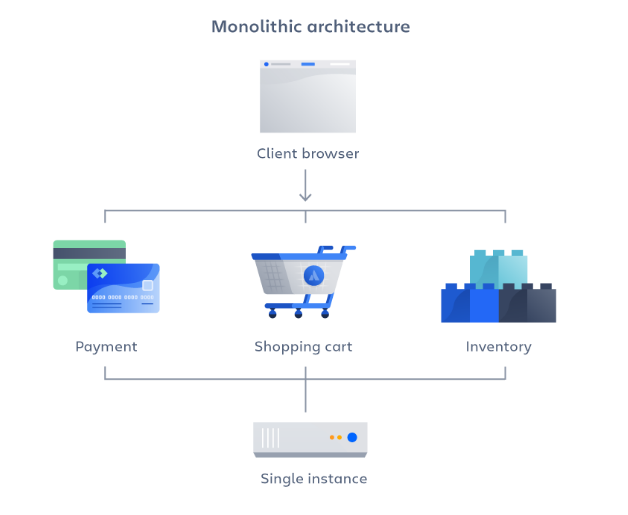
\includegraphics[width=15cm]{graphics/background-knowledge/monolithic-architecture.png}
    \caption{Monolithic Architecture}
    \label{fig:Monolithic Architecture}
\end{figure}

\subsubsection{Multi-tenant Architecture}
Multi-tenancy refers to an architecture where a single instance of software serves multiple customers (tenants) \cite{bezemer2010multitenant}. Each tenant's data is isolated from other tenants, though they share the application and database infrastructure.

In our implementation, we utilize schema-based multi-tenancy within PostgreSQL, where:
\begin{itemize}
    \item Each freight forwarding company occupies a separate database schema
    \item Common application code serves all tenants
    \item Configuration data is tenant-specific
    \item Authentication mechanisms ensure proper data isolation
\end{itemize}

This approach enables our system to serve multiple freight forwarding companies efficiently while maintaining strict data privacy and separation.

\subsection{Web Application Technologies}
\subsubsection{Application Programming Interfaces (APIs)}
APIs serve as intermediary protocols that enable different software applications to communicate with each other. In modern web development, RESTful APIs have become the standard for building interoperable systems \cite{masse2011rest}.

For our freight forwarding system, we implement RESTful APIs characterized by:
\begin{itemize}
    \item Statelessness: Each request contains all information needed for processing
    \item Resource-based routing: Clear endpoint organization based on business entities
    \item Standard HTTP methods: Using GET, POST, PUT, DELETE for CRUD operations
    \item JSON data format: Lightweight data interchange for client-server communication
\end{itemize}

This API design facilitates seamless communication between our frontend and backend components while providing the foundation for potential third-party integrations in future system iterations.

\subsubsection{Single Page Applications (SPA)}
Single Page Applications represent a modern web development approach where the entire application loads a single HTML page and dynamically updates content as users interact with the application \cite{mikowski2013spa}. This paradigm:

\begin{itemize}
    \item Reduces server load by transferring rendering responsibilities to the client
    \item Provides a more responsive user experience with minimized page reloads
    \item Enables rich, desktop-like application behaviors in web browsers
\end{itemize}

Our freight forwarding system utilizes the SPA approach through React.js, allowing for a seamless user experience when navigating between different system modules like quotation management, shipment tracking, and landing page customization.

\subsection{Data Management Concepts}
\subsubsection{Object-Relational Mapping (ORM)}
ORM is a programming technique that connects object-oriented programming languages with relational databases by creating a "virtual object database". This approach:

\begin{itemize}
    \item Abstracts database interactions through programming language objects
    \item Reduces boilerplate SQL code and potential for SQL injection
    \item Facilitates database schema evolution alongside application development
\end{itemize}

In our implementation, we utilize JPA/Hibernate for the backend, enabling efficient database operations while maintaining a clean, object-oriented code structure.

\subsubsection{Database Design for Multi-tenancy}
Implementing multi-tenancy at the database level requires careful consideration of data isolation, performance, and maintenance. Our system employs PostgreSQL schema-based separation, which offers:

\begin{itemize}
    \item Logical separation of tenant data without requiring separate database instances
    \item Efficient resource utilization compared to database-per-tenant approaches
    \item Simplified backup and restoration procedures
    \item Reduced operational overhead while maintaining security boundaries
\end{itemize}

This approach aligns with our requirements for data isolation while providing cost-effective scaling as our user base grows.

\subsection{User Experience Concepts}
\subsubsection{Responsive Design}
Responsive design ensures that web applications render effectively across various devices and screen sizes \cite{marcotte2011responsive}. For a freight forwarding system accessed by users on diverse devices, this approach:

\begin{itemize}
    \item Adapts layout and content based on viewport dimensions
    \item Ensures usability from desktop workstations to mobile devices
    \item Maintains consistent branding and user experience across platforms
\end{itemize}

Our implementation leverages the responsive capabilities of modern CSS frameworks to deliver an adaptive experience optimized for various usage contexts.

\subsubsection{Progressive Enhancement}
Progressive enhancement is a design philosophy that emphasizes core content and functionality first, then progressively adds more complex layers of presentation and features based on browser capabilities \cite{developer_mozilla}. This approach:

\begin{itemize}
    \item Ensures basic functionality remains accessible even in limited environments
    \item Delivers enhanced experiences to users with modern browsers
    \item Supports the diverse technological landscape of global freight operations
\end{itemize}

By adopting progressive enhancement principles, our system remains functional across the varied technical environments common in the logistics industry while delivering optimal experiences where possible.

\section{Foundational Technologies}
\subsection{Programming Languages and Web Technologies}
\subsubsection{Java}
\textbf{Introduction:} Java \cite{java-definition} is a class-based, object-oriented programming language designed to have minimal implementation dependencies. It follows the "write once, run anywhere" (WORA) principle, allowing compiled Java code to run on all platforms that support Java without recompilation.
\textbf{Purpose of use:} In our project, Java serves as the primary backend programming language, providing a robust foundation for implementing business logic, data processing, and integration with external systems. Its enterprise-grade capabilities support the complex operations required in freight management.

\textbf{Advantages:}
\begin{itemize}
    \item Platform independence through the Java Virtual Machine
    \item Strong typing system that reduces runtime errors
    \item Comprehensive standard libraries and frameworks
    \item Robust security features for handling sensitive logistics data
    \item Excellent documentation and large developer community
\end{itemize}

\textbf{Disadvantages:}
\begin{itemize}
    \item Relatively verbose syntax compared to more modern languages
    \item Higher memory consumption than some alternatives
    \item Longer startup times that can impact development speed
    \item Steeper learning curve for beginners
\end{itemize}

\textbf{Ability to meet project requirements:}
\begin{itemize}
    \item Provides the reliability needed for critical shipping operations
    \item Supports complex business rules implementation for freight forwarding
    \item Enables secure handling of sensitive customer and shipment data
    \item Integrates well with enterprise systems common in logistics
\end{itemize}

\subsubsection{HTML/CSS/JavaScript}
\textbf{Introduction:} HTML (HyperText Markup Language) \cite{html5}, CSS (Cascading Style Sheets) \cite{css}, and JavaScript \cite{js} form the core technologies for web development. HTML provides structure, CSS handles presentation, and JavaScript enables interactivity and dynamic content.

\textbf{Purpose of use:} For our freight forwarding system, these technologies create the foundation of our user interface, enabling us to build an accessible, responsive web application that works across various devices used in logistics operations.

\textbf{Advantages:}
\begin{itemize}
    \item Universal browser support ensures wide accessibility
    \item Separation of concerns improves maintainability
    \item Responsive design capabilities adapt to different screen sizes
    \item Rich interactive capabilities through JavaScript
\end{itemize}

\textbf{Disadvantages:}
\begin{itemize}
    \item Browser compatibility issues can increase development complexity
    \item CSS management becomes challenging as applications scale
    \item JavaScript without type checking can lead to runtime errors
    \item Performance optimization requires careful implementation
\end{itemize}

\textbf{Ability to meet project requirements:}
\begin{itemize}
    \item Enables creation of interfaces for various logistics workflows
    \item Supports responsive design for field and office use cases
    \item Provides the interactivity needed for shipment tracking and status updates
    \item Allows progressive enhancement for varying connectivity scenarios
\end{itemize}

\subsubsection{TypeScript}
\textbf{Introduction:} TypeScript \cite{ts} is a strongly typed programming language that builds on JavaScript by adding static type definitions. It compiles to plain JavaScript but provides better tooling and error catching during development.

\textbf{Purpose of use:} In our system, TypeScript enhances JavaScript development by providing type safety and better code organization, which is critical for the complex data structures involved in freight management.

\textbf{Advantages:}
\begin{itemize}
    \item Static typing catches errors during development
    \item Enhanced IDE support with better autocompletion
    \item Improved code documentation through type definitions
    \item Easier refactoring and maintenance for large codebases
\end{itemize}

\textbf{Disadvantages:}
\begin{itemize}
    \item Additional compilation step compared to plain JavaScript
    \item Learning curve for developers unfamiliar with static typing
    \item Type definitions can add verbosity to code
    \item Integration with some third-party libraries may require additional type definitions
\end{itemize}

\textbf{Ability to meet project requirements:}
\begin{itemize}
    \item Ensures data integrity in complex shipping and rate calculations
    \item Improves maintainability for our logistics workflow implementations
    \item Enables safer refactoring as requirements evolve
    \item Provides better documentation for the development team
\end{itemize}

\subsection{Development Frameworks}
\subsubsection{Spring Boot}
\textbf{Introduction:} Spring Boot \cite{spring_boot} is an extension of the Spring framework that simplifies Java application development through convention-over-configuration. It provides a set of pre-configured templates and tools to accelerate development.

\textbf{Purpose of use:} For our freight forwarding system, Spring Boot provides the backend framework that handles API endpoints, business logic, and database operations with minimal boilerplate code.

\textbf{Advantages:}
\begin{itemize}
    \item Rapid development through auto-configuration
    \item Built-in security features for protecting sensitive freight data
    \item Comprehensive testing support for business logic validation
    \item Production-ready monitoring and health checks
\end{itemize}

\textbf{Disadvantages:}
\begin{itemize}
    \item Learning curve for developers new to the Spring ecosystem
    \item "Magic" configuration can be difficult to troubleshoot
    \item Potential overhead for simpler applications
    \item Occasional version compatibility issues with dependencies
\end{itemize}

\textbf{Ability to meet project requirements:}
\begin{itemize}
    \item Provides secure, robust API endpoints for freight operations
    \item Supports complex business logic implementation for shipping processes
    \item Enables efficient database operations for logistics data
    \item Facilitates integration with external shipping and customs services
\end{itemize}

\subsubsection{Node.js}
\textbf{Introduction:} Node.js \cite{nodejs-intro} is an open-source, cross-platform JavaScript runtime environment that executes JavaScript code outside a web browser, using the V8 JavaScript engine.

\textbf{Purpose of use:} In our project, Node.js supports the frontend development environment and certain backend services, providing a JavaScript runtime for server-side execution and build tooling.

\textbf{Advantages:}
\begin{itemize}
    \item Event-driven, non-blocking I/O model for efficiency
    \item Unified language across development stack reduces context switching
    \item Extensive package ecosystem through NPM
    \item Strong community support and frequent updates
\end{itemize}

\textbf{Disadvantages:}
\begin{itemize}
    \item Single-threaded architecture can limit CPU-intensive tasks
    \item Callback patterns can lead to complex code structure
    \item Asynchronous programming model has a learning curve
    \item Evolving ecosystem can lead to dependency management challenges
\end{itemize}

\textbf{Ability to meet project requirements:}
\begin{itemize}
    \item Provides efficient development tools for frontend implementation
    \item Supports asynchronous operations needed for shipping status updates
    \item Enables rapid API prototyping during development
    \item Integrates well with modern web development workflows
\end{itemize}

\subsubsection{React.js}
\textbf{Introduction:} React.js \cite{reactjs} is a JavaScript library for building user interfaces, focusing on component-based architecture and efficient rendering through a virtual DOM implementation.

\textbf{Purpose of use:} In our freight forwarding system, React provides the foundation for our user interface, enabling us to create reusable components that match logistics workflows and efficiently update based on data changes.

\textbf{Advantages:}
\begin{itemize}
    \item Component-based architecture promotes reusability
    \item Virtual DOM ensures efficient UI updates
    \item Unidirectional data flow simplifies state management
    \item Rich ecosystem with many supporting libraries
\end{itemize}

\textbf{Disadvantages:}
\begin{itemize}
    \item Focuses only on UI layer, requiring additional libraries for routing and state management
    \item Learning curve for concepts like JSX and component lifecycle
    \item Regular API changes can require adaptation
    \item Bundle size management requires attention
\end{itemize}

\textbf{Ability to meet project requirements:}
\begin{itemize}
    \item Enables creation of complex, interactive shipping interfaces
    \item Supports efficient updates for real-time tracking features
    \item Allows modular development matching freight forwarding workflows
    \item Provides performance optimizations for data-heavy logistics screens
\end{itemize}

\subsubsection{Next.js}
\textbf{Introduction:} Next.js \cite{nextjs} is a React framework that provides server-side rendering, static site generation, and additional features like routing and API endpoints to enhance React applications.

\textbf{Purpose of use:} For our system, Next.js extends React's capabilities with improved performance, simplified routing, and server-side rendering for better initial page loads.

\textbf{Advantages:}
\begin{itemize}
    \item Server-side rendering improves initial load performance and SEO
    \item Built-in routing system simplifies navigation implementation
    \item Automatic code splitting reduces bundle sizes
    \item API routes enable backend functionality within the same project
\end{itemize}

\textbf{Disadvantages:}
\begin{itemize}
    \item More complex deployment than pure client-side React
    \item Additional build step can slow development iteration
    \item Some React libraries require adaptation for Next.js
    \item Server-side rendering adds complexity to component design
\end{itemize}

\textbf{Ability to meet project requirements:}
\begin{itemize}
    \item Improves load performance for logistics dashboards with large datasets
    \item Simplifies navigation between different freight management sections
    \item Enhances SEO for public-facing freight service pages
    \item Provides consistent structure for large-scale application development
\end{itemize}

\subsubsection{Ant Design}
\textbf{Introduction:} Ant Design \cite{ant-design} is a design system and React UI library that provides a comprehensive set of high-quality components for building enterprise applications.

\textbf{Purpose of use:} In our freight forwarding system, Ant Design provides pre-built UI components that follow enterprise design patterns, accelerating development and ensuring consistency.

\textbf{Advantages:}
\begin{itemize}
    \item Enterprise-focused components suitable for logistics applications
    \item Comprehensive component set reduces development time
    \item Consistent design language throughout the application
    \item Responsive layouts adapt to different device sizes
\end{itemize}

\textbf{Disadvantages:}
\begin{itemize}
    \item Distinctive visual style may require customization
    \item Large component library can increase initial bundle size
    \item Some advanced components have steep learning curves
    \item Customization can become complex for highly specific needs
\end{itemize}

\textbf{Ability to meet project requirements:}
\begin{itemize}
    \item Provides data tables needed for shipping manifests and rate sheets
    \item Offers form components for complex logistics data entry
    \item Includes visualization tools for shipment tracking and analytics
    \item Supports professional presentation required for enterprise logistics
\end{itemize}

\subsection{Database and Storage Technologies}
\subsubsection{PostgreSQL}
\textbf{Introduction:} PostgreSQL \cite{postgres} is an advanced, open-source object-relational database system with a strong reputation for reliability, feature robustness, and performance.

\textbf{Purpose of use:} As our primary database, PostgreSQL stores and manages all freight forwarding data including shipments, clients, rates, and documentation.

\textbf{Advantages:}
\begin{itemize}
    \item Strong support for complex data types and relationships
    \item Advanced indexing and query optimization
    \item Robust transaction support ensures data integrity
    \item Schema-based multitenancy capabilities
\end{itemize}

\textbf{Disadvantages:}
\begin{itemize}
    \item More complex setup and administration than some alternatives
    \item Higher resource requirements than lightweight databases
    \item Horizontal scaling requires additional configuration
    \item Learning curve for advanced features
\end{itemize}

\textbf{Ability to meet project requirements:}
\begin{itemize}
    \item Handles complex relationships between shipments, routes, and documentation
    \item Provides transaction support for critical freight operations
    \item Supports geographic data types for shipping routes and locations
    \item Offers schema separation for multi-tenant freight forwarding companies
\end{itemize}

\subsubsection{Redis}
\textbf{Introduction:} Redis \cite{redis} is an open-source, in-memory data structure store that can be used as a database, cache, and message broker. It supports various data structures and offers optional persistence.

\textbf{Purpose of use:} In our system, Redis provides high-performance caching for frequently accessed data, session management, and temporary storage needs.

\textbf{Advantages:}
\begin{itemize}
    \item Exceptional performance for data retrieval operations
    \item Support for various data structures beyond simple key-value
    \item Built-in expiration policies for cache management
    \item Pub/sub capabilities for real-time features
\end{itemize}

\textbf{Disadvantages:}
\begin{itemize}
    \item In-memory nature limits storage capacity
    \item Potential data loss during crashes if persistence isn't configured
    \item More complex clustering compared to some alternatives
    \item Requires careful memory management
\end{itemize}

\textbf{Ability to meet project requirements:}
\begin{itemize}
    \item Accelerates access to frequently used shipping rates and location data
    \item Provides session storage for user authentication
    \item Supports real-time notifications for shipment status changes
    \item Enables fast search suggestions for logistics entities
\end{itemize}

\subsection{Security and Authentication}
\subsubsection{JSON Web Tokens (JWT)}
\textbf{Introduction:} JWT \cite{jwt} is an open standard that defines a compact and self-contained way for securely transmitting information between parties as a JSON object. The information can be verified and trusted because it is digitally signed.

\textbf{Purpose of use:} Our system uses JWT for authentication and authorization, securing API endpoints and maintaining user sessions without server-side state.

\textbf{Advantages:}
\begin{itemize}
    \item Stateless authentication reduces server storage requirements
    \item Compact format for efficient transmission
    \item Contains user claims and roles for authorization
    \item Works well across services and domains
\end{itemize}

\textbf{Disadvantages:}
\begin{itemize}
    \item Tokens cannot be revoked before expiration
    \item Security depends on proper key management
    \item Token size increases with more claims
    \item Requires secure storage on client side
\end{itemize}

\textbf{Ability to meet project requirements:}
\begin{itemize}
    \item Provides secure access to freight management features
    \item Supports role-based permissions for staff, admin, and client accounts
    \item Enables stateless authentication for scalable deployment
    \item Facilitates secure API access for third-party integrations
\end{itemize}

\subsection{Infrastructure and Deployment}
\subsubsection{Docker}
\textbf{Introduction:} Docker \cite{docker} is a platform that uses OS-level virtualization to deliver software in packages called containers. Containers are isolated from one another and bundle their own software, libraries, and configuration files.

\textbf{Purpose of use:} For our freight forwarding system, Docker provides consistent development and deployment environments, simplifying the transition between stages and ensuring reliable operation.

\textbf{Advantages:}
\begin{itemize}
    \item Environment consistency eliminates configuration discrepancies
    \item Isolation improves security and simplifies dependency management
    \item Resource efficiency compared to traditional virtualization
    \item Simplified deployment and scaling procedures
\end{itemize}

\textbf{Disadvantages:}
\begin{itemize}
    \item Learning curve for developers new to containerization
    \item Potential performance overhead in some scenarios
    \item Storage management for images and volumes
    \item Additional complexity in networking configuration
\end{itemize}

\textbf{Ability to meet project requirements:}
\begin{itemize}
    \item Ensures consistent behavior across development and production
    \item Simplifies deployment of complex freight forwarding components
    \item Provides isolation for multi-tenant configurations
    \item Enables efficient resource utilization for cost-effective hosting
\end{itemize}

\subsection{Development and Collaboration Tools}
\subsubsection{GitHub}
\textbf{Introduction:} GitHub \cite{github} is a web-based platform for version control and collaboration that uses Git as its core technology. It provides hosting for software development and offers distributed version control functionality.

\textbf{Purpose of use:} For our project, GitHub manages source code, facilitates collaboration through code reviews, and tracks issues throughout the development lifecycle.

\textbf{Advantages:}
\begin{itemize}
    \item Comprehensive version control with branching and merging
    \item Pull request workflow supports code quality
    \item Issue tracking integrates with development activities
    \item Documentation capabilities through wikis and README files
\end{itemize}

\textbf{Disadvantages:}
\begin{itemize}
    \item Learning curve for team members new to Git
    \item Potential for merge conflicts in active development
    \item Limited access control options in free tier
    \item Requires internet connectivity for most operations
\end{itemize}

\textbf{Ability to meet project requirements:}
\begin{itemize}
    \item Supports collaborative development across team members
    \item Provides version history for complex freight system components
    \item Enables code review processes to maintain quality
    \item Tracks features and bugs throughout the development lifecycle
\end{itemize}

\subsubsection{Jira}
\textbf{Introduction:} Jira \cite{what-is-jira} is a proprietary issue tracking product developed by Atlassian that allows bug tracking, agile project management, and custom workflow creation.

\textbf{Purpose of use:} In our development process, Jira organizes tasks, tracks progress, and facilitates agile project management for our freight forwarding system.

\textbf{Advantages:}
\begin{itemize}
    \item Flexible workflow customization for different development processes
    \item Comprehensive reporting and visualization tools
    \item Integration with development tools for traceability
    \item Supports agile methodologies like Scrum and Kanban
\end{itemize}

\textbf{Disadvantages:}
\begin{itemize}
    \item Complex interface can be overwhelming for new users
    \item Requires consistent maintenance to remain effective
    \item Configuration complexity for custom workflows
    \item Potential for over-formalization of processes
\end{itemize}

\textbf{Ability to meet project requirements:}
\begin{itemize}
    \item Provides structured tracking of freight system features
    \item Enables clear visualization of development progress
    \item Supports prioritization of critical logistics functionality
    \item Facilitates efficient task assignment and tracking
\end{itemize}